68. $\cfrac{(1-x^2)(x-1)^2(x+1)^3}{x^6-x^4+x^2}\leqslant0\Leftrightarrow\cfrac{-(x-1)^3(x+1)^4}{x^2(x^4-x^2+1)}\leqslant0.$ Применив метод интервалов, найдём ответ: $x\in\{-1\}\cup[1;+\infty).$
\begin{figure}[ht!]
\center{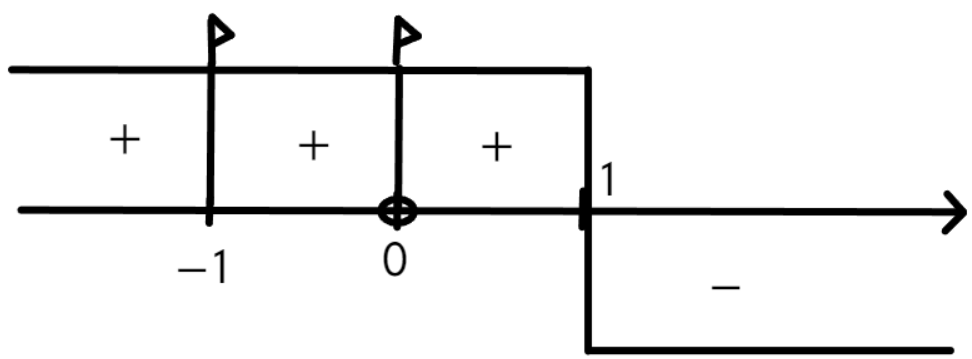
\includegraphics[scale=0.35]{ner9-32.png}}
\end{figure}\\
